\documentclass{beamer}

\usepackage{amsmath, amssymb, hyperref, graphics, wasysym, tikz}
%\usetikzlibrary{cd}
\usepackage{mathpazo}

\AtBeginDocument{
   \DeclareSymbolFont{AMSb}{U}{msb}{m}{n}
   \DeclareSymbolFontAlphabet{\mathbb}{AMSb}}

\newcommand{\AAA}{\mathbb{A}}
\newcommand{\C}{\mathbb{C}}
\newcommand{\Z}{\mathbb{Z}}
\newcommand{\R}{\mathbb{R}}
\newcommand{\Q}{\mathbb{Q}}

\title{MAS439 Lecture 14 \\ Coordinate Ring}

\date{November 23rd}

\begin{document}

\begin{frame}
\titlepage
\end{frame}


 \begin{frame}{Where we are:}

We've seen that the maps $V$ and $I$ are inverse to each other and set up 1:1 correspondences between certain types of ideals in $R=k[x_1,\dots, x_n]$ and certain types of subsets of $\AAA^n_k$.

\begin{center}
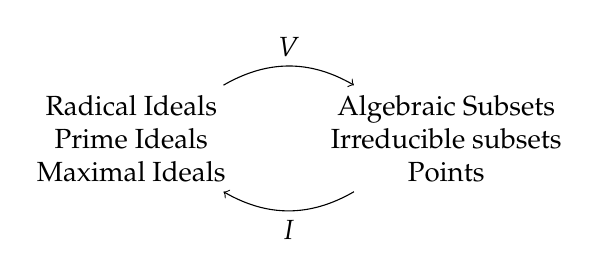
\begin{tikzpicture}

\node[align=center]  (a) at (0,0) {Radical Ideals \\ Prime Ideals \\ Maximal Ideals };
\node[align=center] (b) at (4,0) {Algebraic Subsets \\ Irreducible subsets  \\ Points};

\draw[->] (a) edge[bend left] node[above] {$V$} (b);
\draw[->] (b) edge[bend left] node[below] {$I$} (a);
\end{tikzpicture}
\end{center}


\end{frame}


\begin{frame}{What's next?}


The correspondence above holds for ideals of $k[x_1,\dots, x_n]$, which is a very special example of a $k$-algebra.  We'd like a geometric way to study the ideals of other rings. \\~\\

We've seen that any finitely generated reduced $k$-algebra $S$, we have $S\cong k[x_1,\dots, x_n]/I$ for some $n$ and radical ideal $I$.  \\~\\

Today we will see that we can view $S=k[x_1,\dots, x_n]/I$ as functions on the algebraic subset $V(I)$: we will call $S$ the \emph{coordinate ring of $V(I)$}, and that ideals of $S$ will be related to the geometry of $V(I)$.  \\~\\

Tomorrow, we will study maps between different algebraic subsets, and how they relate to maps between their coordinate rings.

\end{frame}


\begin{frame}{The Coordinate ring}

\begin{definition}
Let $X\subset \AAA_k^n$ be an algebraic subset.  The \emph{coordinate ring} $k[X]$ of $X$ is defined to be the quotient ring 

$$k[X]=k[x_1,\dots, x_n]/I(X)$$
\end{definition}

Since $I(X)$ is always radical, the coordinate ring $k[X]$ is always reduced. \\~\\

Since $k[x_1,\dots, x_n]$ is a $k$-algebra, so is $k[X]$. 
\begin{block}{How is $k[X]$ related to $X$?}
\end{block}

\end{frame}

\begin{frame}{Polynomial Functions}

We can view the polynomial ring $R=k[x_1,\dots, x_n]$ as a subring of the space of all functions from $\AAA_k^n$ to $k$.  \\~\\

If $X\subset \AAA_k^n$, then we can also view a polynomial as a function on $X$.


\begin{definition}
Let $X\subset \AAA__k^n$ be algebraic.  We call a function $f:X\to k$ \emph{polynomial} if there is a polynomial $g\in R=k[x_1,\dots, x_n]$ so that $f(x)=g(x)$ for all $x\in X$. 
\end{definition}

Let $\text{Fun}_{\text{poly}}(X)$ denote the set of all polynomial functions on $X$.   

\begin{block}{Claim:}
$\text{Fun}_{\text{poly}}(X)$ is a $k$-algebra
\end{block}

\end{frame}


\begin{frame}{The coordinate ring is the polynomial functions}

\begin{lemma}
Let $X\subset \AAA_k^n$ algebraic.  Then 
$$k[X]:=k[x_1,\dots, x_n]/I(X)\cong \text{Fun}_{\text{poly}}(X)$$
\end{lemma}

\begin{proof}
\begin{itemize}
\item The restriction map $\textrm{Res}:R=k[x_1,\dots, x_n]\to \textrm{Fun}_{\textrm{poly}}(X)$ is a homomorphism, and is surjective by definition.
\item A polynomial $f\in R$ is in the kernel of $\textrm{Res}$ is equivalent to $f(x)=0$ for all $x\in X$; that is, that $f(x)\in I(X)$.
\item The first isomorphism theorem then says that $\textrm{Fun}_{\textrm{poly}}(X)\cong R/I(X)$, as desired.
\end{itemize}
\end{proof}

\end{frame}


\begin{frame}{Geometry and the Ideals of $K(X)$}

Since $K(X)=R/I(X)$, the second isomorphism theorem says that ideals in $K(X)$ are in 1-1 correspondence with ideals of $R$ containing $I(X)$. \\~\\

Since $I$ is inclusion reversing, we see that radical ideals of $K(X)$ are in 1-1 correspondence with algebraic subsets of $\AAA_k^n$ contained in $X$. \\~\\

\begin{center}
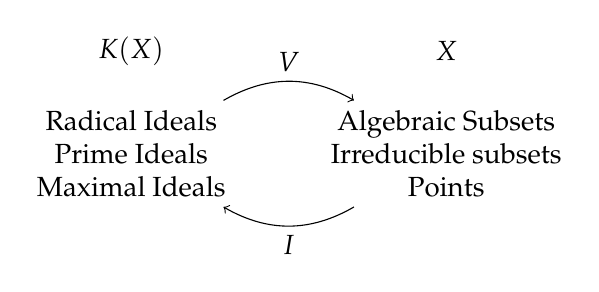
\begin{tikzpicture}

\node[align=center]  (a) at (0,0) {Radical Ideals \\ Prime Ideals \\ Maximal Ideals };
\node[align=center] (b) at (4,0) {Algebraic Subsets \\ Irreducible subsets  \\ Points};

\node at (0,1.3) {\alert{$K(X)$}};
\node at (4,1.3) {\alert{$X$}};
\draw[->] (a) edge[bend left] node[above] {$V$} (b);
\draw[->] (b) edge[bend left] node[below] {$I$} (a);
\end{tikzpicture}
\end{center}


\end{frame}

\begin{frame}{Example:}

Find all the radical/prime/maximal ideals of $R=k[x,y]/(x^2y+xy^2-xy)$.

\begin{block}{Technique:}

We'd like to use the previous slide and relate the ideals to of $R$ to the geometry of $V(x^2y+xy^2-xy)$, but to do this, we must first check that $(x^2y+xy^2-xy)$ is radical. \\~\\

This is not hard as $(x^2y+xy^2-xy)$ is principal and $k[x,y]$ is a unique factorisation domain... 

\end{block}

\end{frame}


\end{document}
